\section{Fixed charge and the two real sections}\label{sec:background}
Let $Y=S^3/\Gamma$ have the induced unit-radius metric, orientation and spin lift, and write $V=2\pi^2/|\Gamma|$. We take signature $(-+++)$ before continuation and choose the trace of torsion as $T^a{}_{ab}$. The real parameter $h=2\kappa^2 c_H$ multiplies the Holst term in the normalization of Paper~08. Set
\begin{equation}
 d=1+h^2,\quad P=Q_\Sigma=-p_\theta,\quad s=\sgn P,\quad c=\frac{|P|}{6V},\quad
 a=\sqrt d\,c=q_*^2,\qquad A_0=\frac{3V}{\kappa^2}.
 \label{eq:scales}
\end{equation}
We take $P\ne0$. The action consists of the Einstein--Cartan term, $\theta\,\dd(e^a\wedge T_a)$, a constant Holst density and the metric boundary term after connection elimination. The trace and axial equations for a homogeneous timelike source give axial coefficient $j=-\kappa^2\dot\theta/d=s c/q^3$ and vector coefficient $-hj$ in proper Lorentzian time. The dimensionless auxiliary connection Hessian has determinant $256d^{12}$. Its Schur complement gives the Lorentzian scalar density $-C(\nabla\theta)^2$ with $C=3\kappa^2/d$. At $h=0$ the canonical scalar is $\sqrt6\,\kappa\theta$; the contortion involves the derivative of $\kappa^2\theta$. In particular the conserved NY charge is distinguished from the integration constant for the field velocity at nonzero $h$.

The homogeneous Legendre transform fixes $p_\theta$, so that the scalar enters the Euclidean action with a positive flux potential. With lapse $N$, proper radial coordinate at $N=1$, induced outer radius $R$ and the flat reference boundary curvature, the action is
\begin{equation}
 I_P=A_0\int\left(-\frac{q\dot q^2}{N}-Nq+\frac{Na^2}{q^3}\right)\dd\tau+A_0 R^2 .
 \label{eq:action}
\end{equation}
The inner reflection surface has zero extrinsic curvature. Varying $N$ before setting it to one gives $\dot q^2=1-a^2/q^4$. Hence the outward proper acceleration at the throat is $2/q_*$. In conformal Euclidean time $\dd\tau=q\,\dd t$ this integrates to
\begin{equation}
 q_E^2=a\cosh(2t),\quad 0\le t\le T,\qquad
 T=\tfrac12\operatorname{arcosh}(R^2/a).
 \label{eq:q}
\end{equation}
The positive Lorentzian slice solves $(\dd q/\dd\tau_L)^2=a^2/q^4-1$ and $q_L^2=a\sin(2u)$ with $\dd\tau_L=q\,\dd u$. Continuation $u=\pi/4-it$ joins the two real metrics at vanishing first derivative. The section which is a maximum in Lorentzian time is the minimum of the real Euclidean radius. The positive Euclidean metric satisfies the complex-metric eigenvalue phase criterion trivially. This metric test does not specify a real contour for axion perturbations about an imaginary scalar derivative.

The closed spatial flux is constant along the regular collar. With the outward boundary orientations its two integrals cancel in the integral of the complete Nieh--Yan derivative. A single mouth therefore carries $P$ without fixing an integer four-dimensional charge on this boundary value problem. Substitution of the constraint into \eqref{eq:action} gives the regulated Hamilton principal function
\begin{equation}
 \frac{I_P(R)}{A_0}
 = R^2-2\int_{q_*}^R q\sqrt{1-a^2/q^4}\,\dd q
 = R^2-\sqrt{R^4-a^2}+a\arccos(a/R^2).
 \label{eq:principal}
\end{equation}
At infinity $I_P^\infty=\pi A_0 a/2=\pi\sqrt d\,|P|/(4\kappa^2)$. At fixed total charge this result is independent of the quotient order; at fixed density it scales with $V$. At fixed $q_*$ the infinite-end action is independent of $h$. At finite, fixed absolute $R$ one must use \eqref{eq:principal}. Changing $R$ together with the throat changes the boundary metric.

\begin{figure}[htbp]
\centering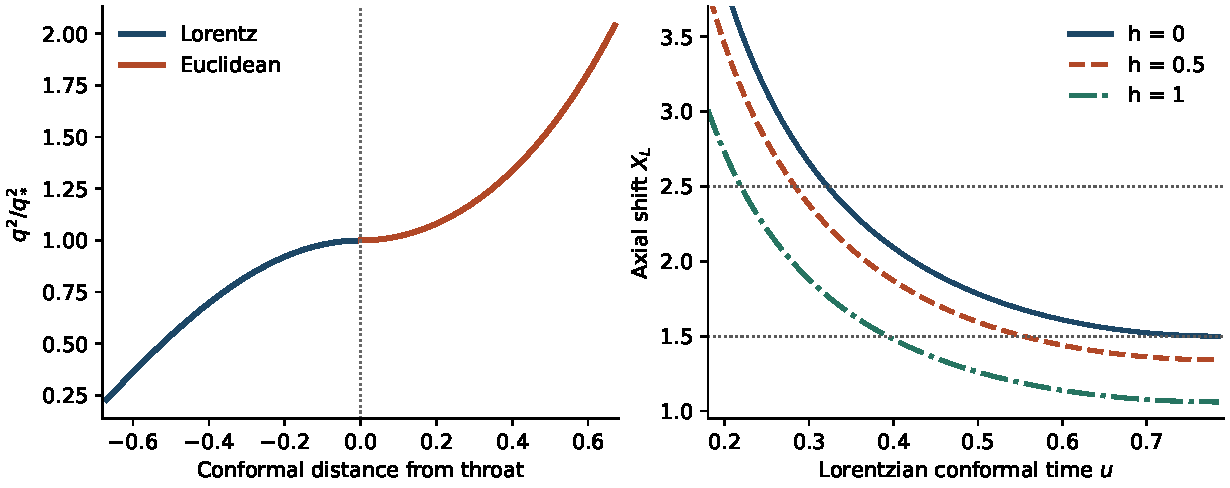
\includegraphics[width=.97\linewidth]{figures/throat.pdf}
\caption{Left: area radius squared in units of $a$ as a function of conformal distance from the reflection surface, with applications to a Lorentzian expansion and an outward Euclidean collar. Right: Lorentzian axial shift for $h=0,1/2,1$. The dashed horizontal lines are the first two absolute shell energies. The interval between the first crossing and the reflection surface is empty at $h=0$.}
\label{fig:throat}
\end{figure}
